\subsection{Electric Motor Model}

The most wide-spread motor used in small UAVs is the brushless outrunner permanent magnet electrical motor. Commonly a 3-constant model is used, but for the sake of completeness, a 4-constant model will be used here, as presented in \cite{Carri2007}. The equivalent circuit can be seen in Figure \ref{fig:motor_electric_4c}, form the same source.

\begin{figure}
	\centering
	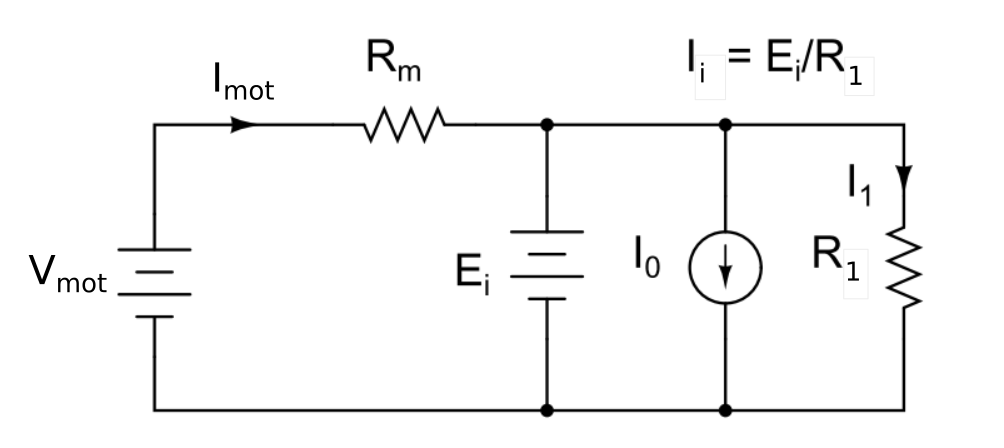
\includegraphics[width=0.7\textwidth]{figures/motor_electric_4c}
	\caption[Coefficient of Thrust as a function of Advance Ratio]{Coefficient of Thrust as a function of Advance Ratio}
	\label{fig:motor_electric_4c}
\end{figure}

The input to the motor is the driving voltage, $V_{mot}$ and the output is the output power, $P_{mot}$. Naturally, if there is a direct-drive configuration between the motor and the propeller, the motor rotational speed ($n_{mot}$, in revolutions per second) is the same as that of the propeller.

\begin{lstlisting}[style=C-style]
	n_prop = n_mot
\end{lstlisting}

\begin{IEEEeqnarray}{rCl}
	n_{mot} &= & K_v E_i \label{eq:motorKV}\\
	E_i &= & V_{mot} - I_{mot} R_m \label{eq:motorRM}\\
	P_{mot} &= & E_i I_i \\
	I_i &= & I_{mot} - I_0 - \frac{E_i}{R_1} \label{eq:motorR1}\\
	P_{elec} &= & V_{mot}I_{mot}
\end{IEEEeqnarray}

\begin{lstlisting}[style=C-style]
	n_mot = K_v*E_i
	E_i = V_mot - I_mot*R_m
	P_mot = E_i*I_i
	I_i = I_mot - I_0 - E_i/R_1
	P_elec = V_mot*I_mot
\end{lstlisting}

\subsection{Battery and Electronic Speed Controller}

Finally, an expression for the overall combination of the battery and ESC is given.
\begin{itemize}
\item $V_{bat}$ is the internal battery voltage
\item $R_{bat}$ is the battery internal resistance
\item $R_S$ is the ESC in-line resistance
\item $\delta_t$ is the throttle command, essentially modulating the output voltage
\end{itemize}

\begin{IEEEeqnarray}{rCl}
	V_{mot} &= & (V_{bat} - I_{mot} (R_{bat} + R_S)) \delta_t \label{eq:battR}
\end{IEEEeqnarray}

\begin{lstlisting}[style=C-style]
	V_mot = (V_bat - I_mot*(R_bat + R_S))*deltat
\end{lstlisting}